% Source page: original p. 344 (PDF p. 40)
% Figure number: Figure 16
% Uncertainty notes: The two potential profiles are reconstructed from the scan and adjacent prose; the broad shapes and asymptotic behavior match the source, while small curvature details remain approximate.
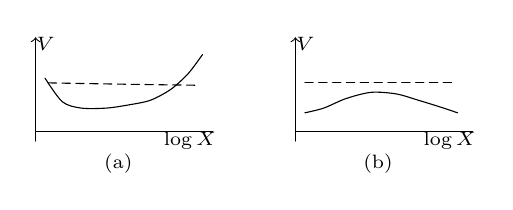
\begin{tikzpicture}[x=1cm,y=1cm,line cap=round,line join=round]
  \begin{scope}
    \draw[->] (0,-0.02) -- (0,1.30);
    \draw (0,0.10) -- (2.25,0.10);
    \node[font=\scriptsize] at (0.13,1.22) {$V$};
    \node[font=\scriptsize] at (1.96,-0.02) {$\log X$};

    \draw[densely dashed] (0.16,0.72) .. controls (0.72,0.71) and (1.25,0.70) .. (2.06,0.69);
    \draw[smooth] plot coordinates {
      (0.12,0.78) (0.34,0.48) (0.58,0.40) (0.90,0.40)
      (1.18,0.44) (1.46,0.50) (1.72,0.64) (1.94,0.84) (2.12,1.08)
    };
    \node[font=\scriptsize] at (1.05,-0.30) {(a)};
  \end{scope}

  \begin{scope}[xshift=3.3cm]
    \draw[->] (0,-0.02) -- (0,1.30);
    \draw (0,0.10) -- (2.25,0.10);
    \node[font=\scriptsize] at (0.13,1.22) {$V$};
    \node[font=\scriptsize] at (1.96,-0.02) {$\log X$};

    \draw[densely dashed] (0.12,0.72) -- (2.04,0.72);
    \draw[smooth] plot coordinates {
      (0.12,0.34) (0.36,0.40) (0.64,0.52) (0.96,0.60)
      (1.28,0.58) (1.56,0.50) (1.82,0.42) (2.06,0.34)
    };
    \node[font=\scriptsize] at (1.05,-0.30) {(b)};
  \end{scope}
\end{tikzpicture}
